%&"pre"
\begin{document}
    \title{B4: Google's Software-Defined WAN}
    \subtitle{Paper Reading}
    \author{Log Creative}
    \date{\today}
    \maketitle
    \begin{frame}
        \frametitle{论文}
        \fullcite{Hong2018}
    \end{frame}

    \section{简介}

    \begin{frame}
        \frametitle{B4}
        \framesubtitle{Google 私有广域网后端}
        \framezoom<1><2>(1cm,1.5cm)(3cm,2cm)
        \begin{figure}
            \centering
            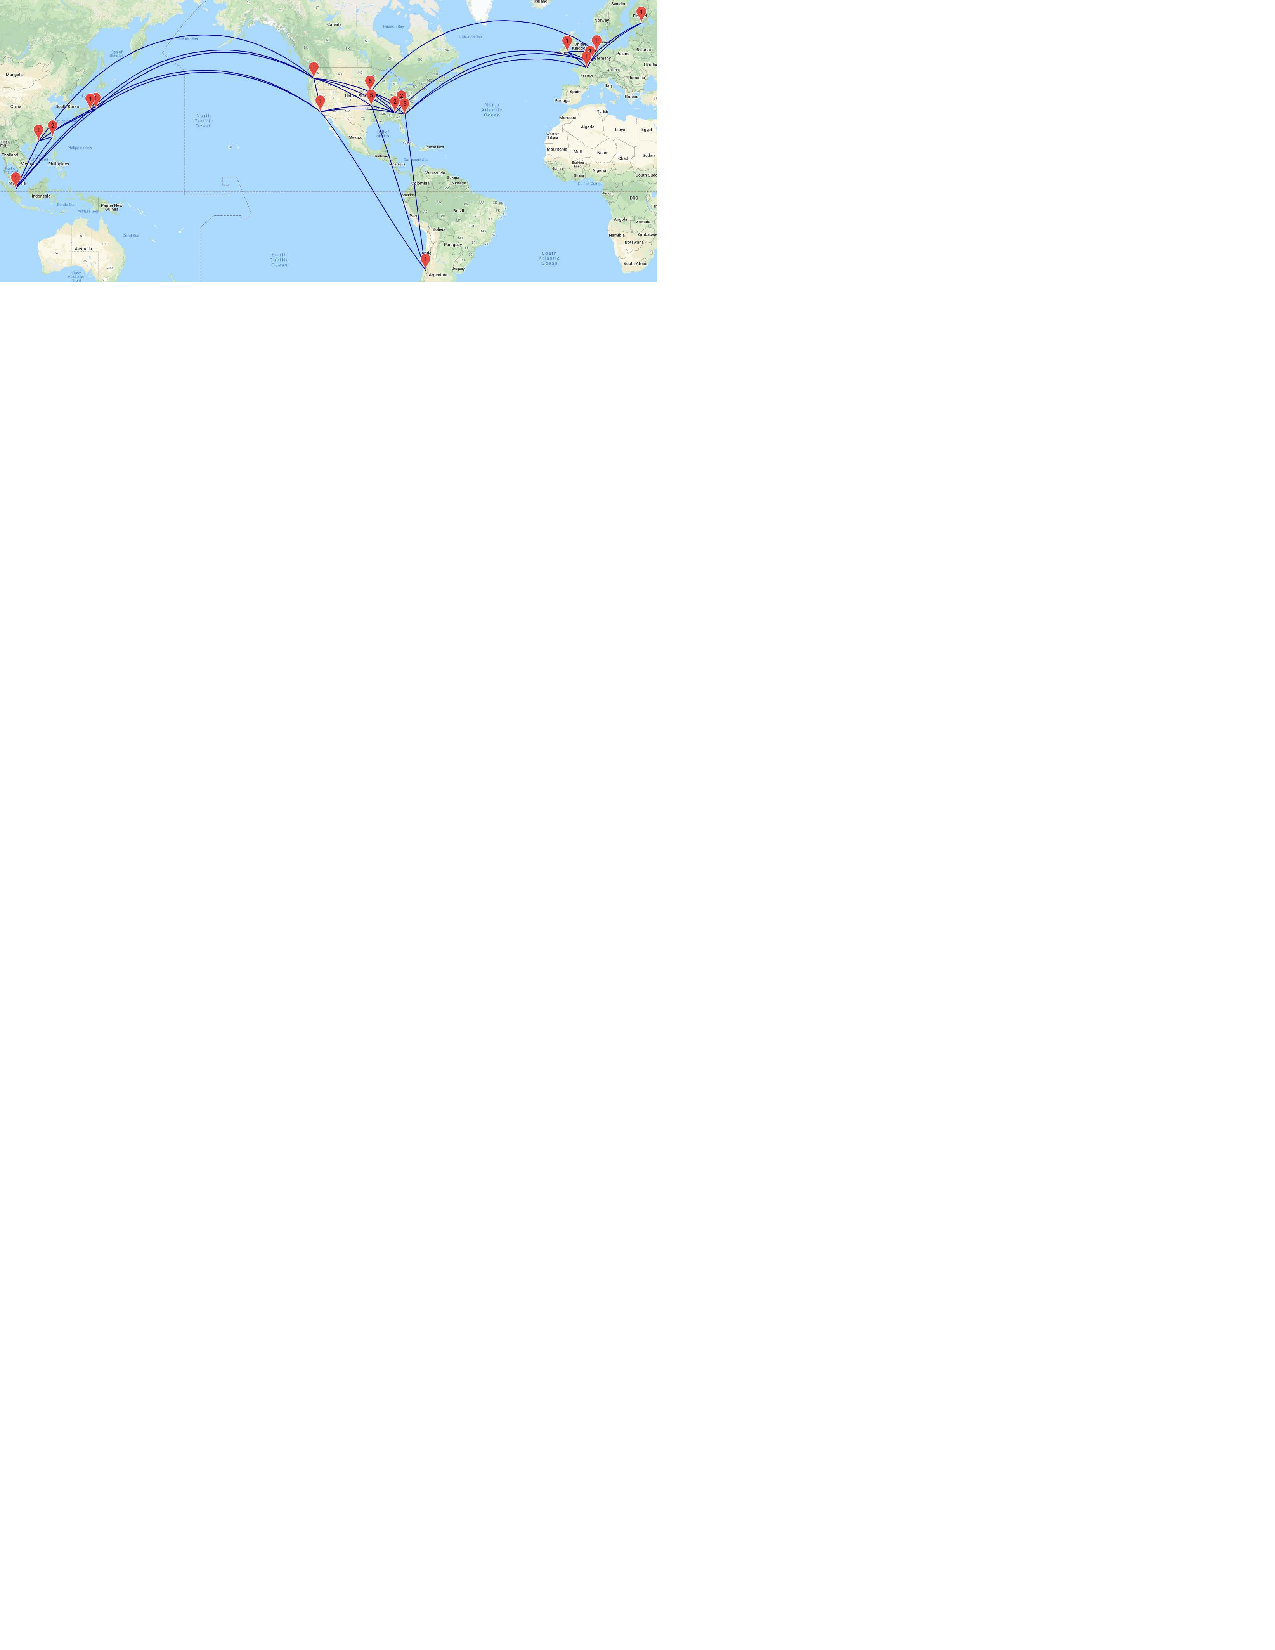
\includegraphics[height=0.6\textheight]{b4.pdf}
            \caption{B4 全球网络}
        \end{figure}
        \only<2>{
            \begin{tikzpicture}[overlay]
                \node [right] at (1cm,4cm) {TE};
                \node [right] at (1cm,3.7cm) {\tiny Traffic};
                \node [right] at (1cm,3.5cm) {\tiny Engineering};
            \end{tikzpicture}
        }
    \end{frame}

    \begin{frame}
        \frametitle{SLO}
        \framesubtitle{Service Level Objectives 服务级别协议}
        表示 30 天滑动窗口内的网络连接可用性和带宽可用性。
        \begin{table}
            \begin{tabular}{clr}
                \toprule
                服务级别 & 应用举例 & SLO需求\\
                \midrule
                \rowcolor<3>{csecondary!30} SC4 & 搜索广告、DNS、WWW & 99.99\%\\
                SC3 & 照片服务后端、邮件 & 99.95\%\\
                SC2 & 广告数据库拷贝 & 99.90\%\\
                SC1 & 搜索索引拷贝 & 99\%\\
                \rowcolor<2>{ctertiary!30} SC0 & 批量传输 & \\
                \bottomrule
            \end{tabular}
            \caption{SLO}
        \end{table}
    \end{frame}

    \section{背景与动机}

    \begin{frame}
        \frametitle{扁平结构}
        \framesubtitle{不利于扩展和可用性}
        之前的 B4 若想增加容量,需要在地理限界内增加站点。但这会带来:
        \begin{enumerate}
            \item 增加了中央流量控制优化算法的运行时间。
            \item 对交换机有限的流表空间增加压力。
            \item 使得容量管理变得复杂并给应用开发者造成麻烦。
        \end{enumerate}
        \only<2>{为了解决这个问题,引入 \emph{supernode} 和两层架构。} % 后文讨论细节
    \end{frame}

    \begin{frame}
        \frametitle{层级架构}
        \framesubtitle{容量不对等问题}
        B4 中 6--20\% 的地理级连接仍然会在 $\geq$ 5\% 的时间内有容量不对等情形。
        \begin{figure}[H]
            \centering
            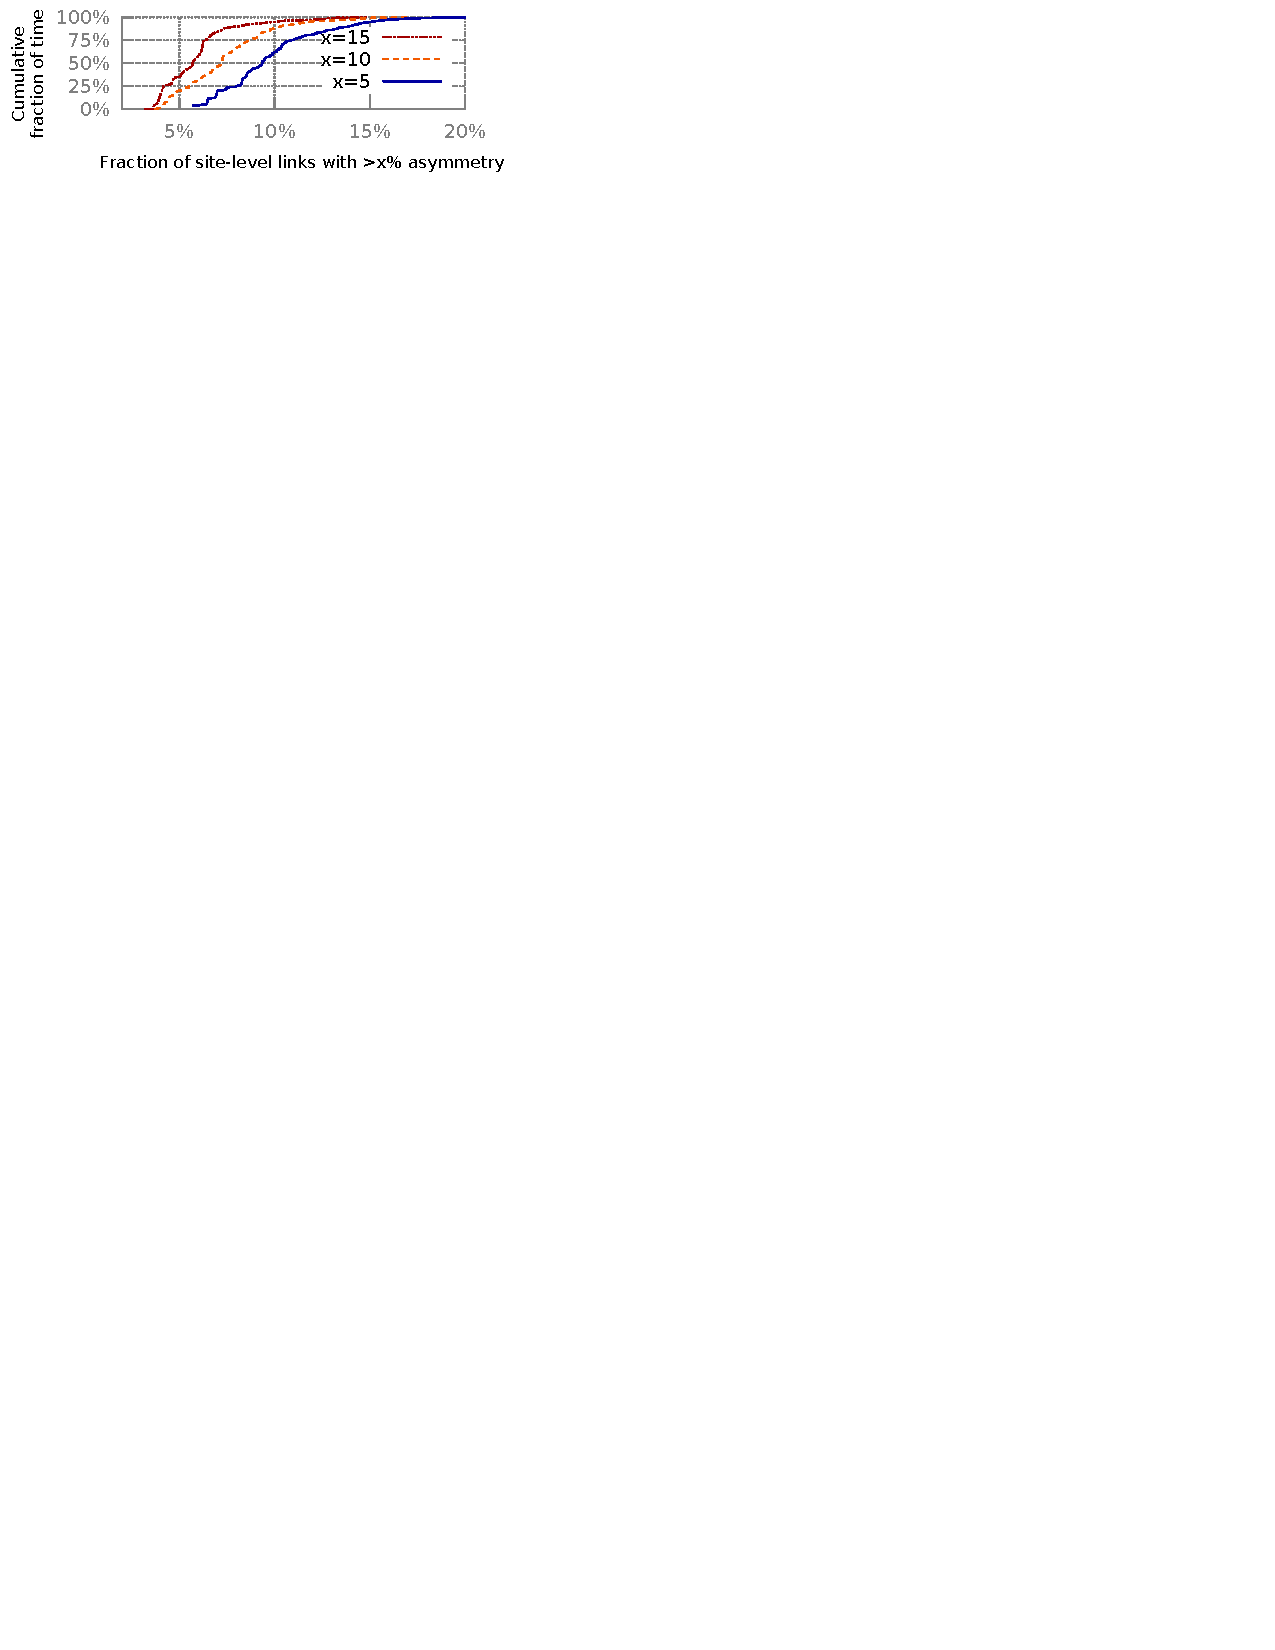
\includegraphics[height=0.5\textheight]{asym}

            $\frac{\text{avg}_{\forall i} C_i - \text{min}_{\forall i} C_i}{\text{avg}_{\forall i} C_i}$
            \caption{地理级流量不对等}\label{fig:asym}
        \end{figure}
    \end{frame}

    \begin{frame}
        \frametitle{不对等的后果}
        \framesubtitle{大幅减少系统效率}

        \begin{figure}
        \centering
        \begin{tikzpicture}
            \tikzstyle{supernode}=[rectangle,draw,minimum width=1.5cm,minimum height=1cm,fill=white];
            \tikzstyle{flow}=[->];
            \draw[draw=none,fill=cprimary!10]  (-1.5,2) rectangle (0.5,-2);
            \draw[draw=none,fill=cprimary!10]  (1.5,2) rectangle (3.5,-2);
            \node[supernode] (a1) at (-0.5,1) {$A_1$};
            \node [supernode] (b1) at (2.5,1) {$B_1$};
            \node [supernode] (b2) at (2.5,-1) {$B_2$};
            \only<1>{
                \node [supernode] (a2) at (-0.5,-1) {$A_2$};
                \draw [flow](-2,-1) node[left]{$\frac{c}{2}$} -- (a2);
            }
            \only<2->{
                \node [supernode,draw=csecondary] (a2) at (-0.5,-1) {\color{csecondary}$A_2$};
                \draw [flow,csecondary](-2,-1) node[left]{\color{csecondary} $\frac{c}{2}$} -- (a2);
            }
            \node at (-0.5,2.5) {Site $A$};
            \node at (2.5,2.5) {Site $B$};
            \draw[flow] (-2,1) node[left] {$\frac{c}{2}$} -- (a1);
            
            \draw (a1) -- (b2);
            \draw  (a1) edge (b1);
            \only<1>{
                \draw (a2) edge node[above] {5} (b1);
                \draw (a2) edge node[above] {5} (b2);
            }
            \only<2->{
                \draw[csecondary] (a2) edge node[above] {1} (b1);
                \draw[csecondary]  (a2) edge node[above] {1} (b2);
            }
            \draw  (b1) edge node [right] {4} (b2);
            \only<3->{
                \draw[cprimary] (a1) edge node [left] {\emph{sidelink}} node[right] {4} (a2);
            }
        \end{tikzpicture}
        \caption{\only<1>{对等} \only<2->{不对等示例} \only<2>{$c=4$} \only<3>{$c=12$}}\label{fig:asymeg}
        \end{figure}
    \end{frame}

    \begin{frame}
        使用 \emph{sidelink} 可以提高不对等时的带宽利用率。但是仍然需要考虑相关的协议问题,比如有些数据不可分割、MAC 地址不可变化,% 后文使用算法解决。
        
        以及死循环问题,转换路径可能是\emph{原子操作},以任意顺序应用 TE 更新会导致这种死循环率上升,% 后文会通过另一种算法完成。
    \end{frame}

    \makebottom
\end{document}